\begin{subfigure}[h]{0.33\textwidth}
    \centering
    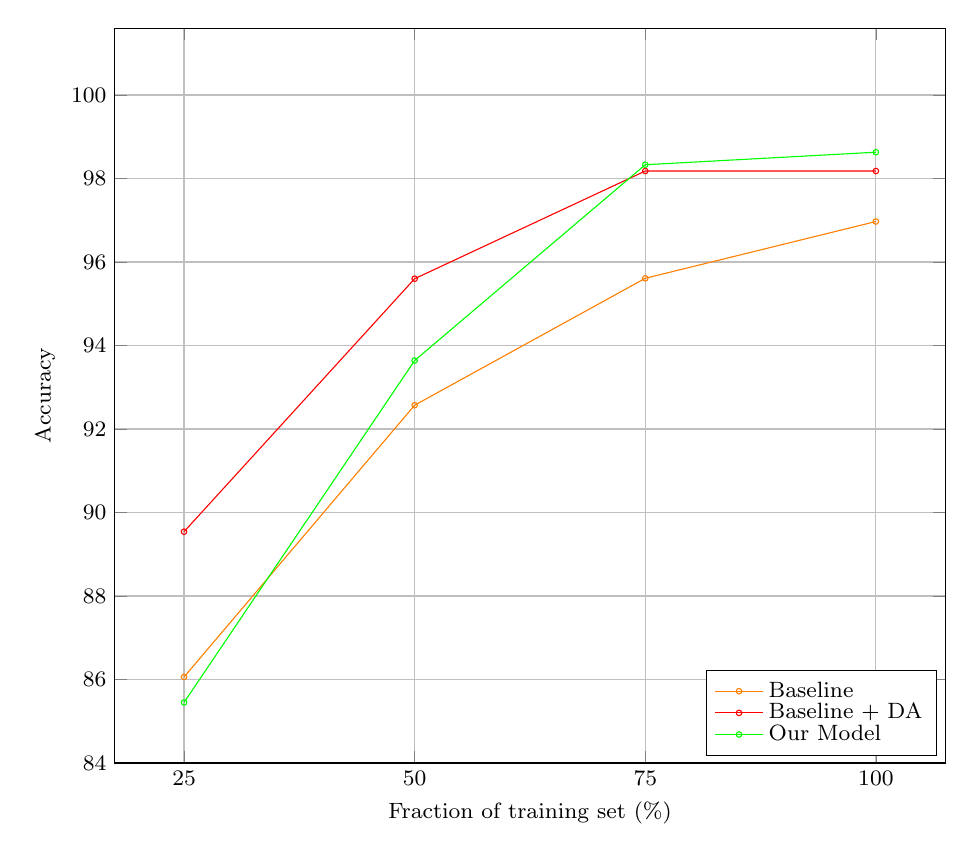
\begin{tikzpicture}[scale=1.0]
      \footnotesize
      \begin{axis}[ 
        legend cell align={left},
        legend style={legend style={row sep=-3pt},
        at={(0.99,0.01)},anchor=south east},
        width=1.0\linewidth,
        height=0.9\linewidth,
        xlabel=Fraction of training set (\%),
        ylabel=Accuracy,
        grid=major,
        % legend pos=south east,
        xlabel near ticks,
        xticklabel style={/pgf/number format/1000 sep=},
        ylabel near ticks,
        xtick=data,
        yticklabel style={
            left,
            /pgf/number format/.cd,
            fixed,
            precision=2,
            /tikz/.cd
        },
        enlarge y limits={value=.1,upper},
        log ticks with fixed point,
        ymin=84,
        ymax=100
      ] 
        % \addplot[color=orange,mark=o, mark options={scale=0.5}] coordinates { (10,69.39) (25, 86.06) (50,92.57) (75,95.61)  (100,96.97)};
        % \addplot[color=red,mark=o, mark options={scale=0.5}] coordinates { (10,74.24) (25,89.54) (50,95.60) (75,98.18) (100,98.18)};
        % \addplot[color=green,mark=o, mark options={scale=0.5}] coordinates { (10,69.24) (25,85.45) (50,93.64) (75,98.33) (100,98.63)};
        \addplot[color=orange,mark=o, mark options={scale=0.5}] coordinates { (25, 86.06) (50,92.57) (75,95.61)  (100,96.97)};
        \addplot[color=red,mark=o, mark options={scale=0.5}] coordinates { (25,89.54) (50,95.60) (75,98.18) (100,98.18)};
        \addplot[color=green,mark=o, mark options={scale=0.5}] coordinates { (25,85.45) (50,93.64) (75,98.33) (100,98.63)};                      
        \legend{Baseline, Baseline + DA, Our Model}
      \end{axis}
    \end{tikzpicture}
    \caption{Only geometric transformations}
    \label{fig_Brain40x_geo}
\end{subfigure}